\documentclass[tikz,border=2pt]{standalone}

\usepackage{pgfplots}
\pgfplotsset{compat=1.18}

% ============================================================
% Color palette
% ============================================================

\definecolor{EmpiricalColor}{HTML}{2A6F6B}
\definecolor{NominalColor}{HTML}{C86442}
\definecolor{AxisColor}{HTML}{46515C}
\definecolor{GridColor}{HTML}{DCE2E6}

\begin{document}

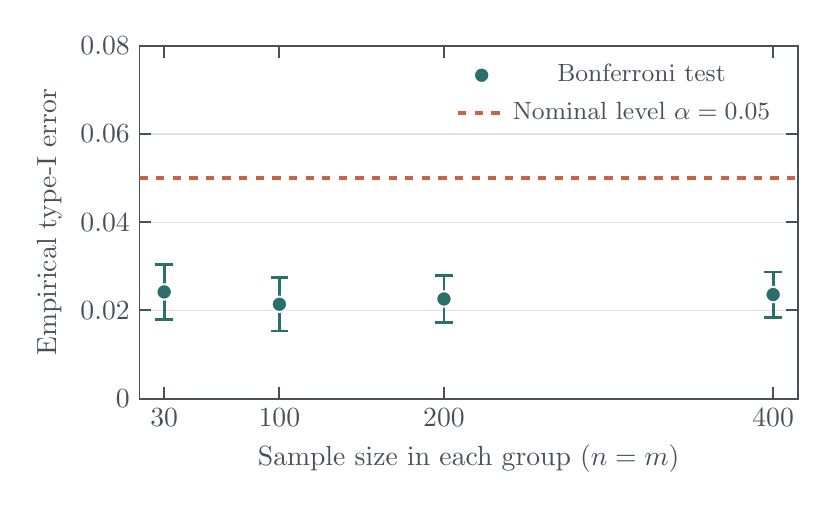
\begin{tikzpicture}
    \begin{axis}[
        width=0.82\linewidth,
        height=0.50\linewidth,
        xlabel={Sample size in each group ($n=m$)},
        ylabel={Empirical type-I error},
        xmin=15,
        xmax=415,
        ymin=0.00,
        ymax=0.08,
        xtick={30,100,200,400},
        ytick={0.00,0.02,0.04,0.06,0.08},
        scaled y ticks=false,
        yticklabel={
            \pgfmathprintnumber[
                fixed,
                precision=2
            ]{\tick}
        },
        axis line style={
            AxisColor,
            line width=0.7pt
        },
        tick style={
            AxisColor,
            line width=0.7pt
        },
        ticklabel style={
            text=AxisColor
        },
        label style={
            text=AxisColor
        },
        ymajorgrids=true,
        xmajorgrids=false,
        grid style={
            GridColor,
            line width=0.5pt
        },
        legend style={
            draw=none,
            fill=none,
            text=AxisColor,
            font=\small,
            at={(0.98,0.98)},
            anchor=north east,
            row sep=2pt
        }
    ]

    % ========================================================
    % Empirical type-I errors and Monte Carlo intervals
    % ========================================================

    \addplot+[ only marks,
        color=EmpiricalColor,
        line width=1.5pt,
        mark=*,
        mark size=2.8pt,
        mark options={
            fill=EmpiricalColor,
            draw=white,
            line width=0.7pt
        },
        error bars/.cd,
        y dir=both,
        y explicit,
        error bar style={
            color=EmpiricalColor,
            line width=1.0pt
        },
        error mark options={
            color=EmpiricalColor,
            rotate=90,
            mark size=3.2pt,
            line width=1.0pt
        }
    ]
    table[
        x=n,
        y=typeI,
        y error=error
    ] {
        n    typeI    error
        30   0.0242   0.006298
        100  0.0214   0.006075
        200  0.0226   0.005286
        400  0.0236   0.005122
    };

    \addlegendentry{Bonferroni test}

    % ========================================================
    % Nominal significance level
    % ========================================================

    \addplot[
        color=NominalColor,
        dashed,
        line width=1.4pt
    ]
    coordinates {
        (15,0.05)
        (415,0.05)
    };

    \addlegendentry{Nominal level $\alpha=0.05$}

    \end{axis}
\end{tikzpicture}

\end{document}